\documentclass{article}
\usepackage{amsmath}
\usepackage{amssymb}
\usepackage{graphicx}
\usepackage{hyperref}
\usepackage[version=4]{mhchem}


\begin{document}
(1995 AMC) In the figure, \(A B\) and \(C D\) are diameters of the circle with center \(O, A B \perp C D\), and chord \(D F\) intersects \(A B\) at \(E\). If \(D E=6\) and \(E F=2\), then the area of the circle is


(A) \(23 \pi\)\\
(B) \(\frac{47}{2} \pi\)\\
(C) \(24 \pi\)\\
(D) \(\frac{49}{2} \pi\)\\
(E) \(25 \pi\)

Solution: (C).\\
Draw segment \(F C\). Angle \(C F D\) is a right angle since arc \(C F D\) is a semicircle. Then right triangles \(D O E\) and \(D F C\) are similar to each other, so the following equality holds true:\\
\(\frac{D O}{D F}=\frac{D E}{D C}\).\\
Let \(D O=r\) and \(D C=2 r\). Substituting this into the equality above, we have \(\frac{r}{8}=\frac{6}{2 r} \quad \Rightarrow \quad 2 r^{2}=48 \quad \Rightarrow\)\\
\centering
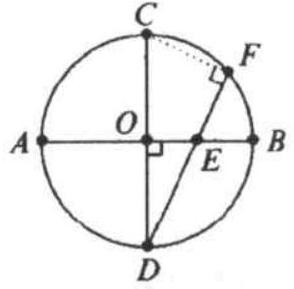
\includegraphics[width=\textwidth]{images/167(1).jpg}

\[
r^{2}=24 .
\]

The area of the circle is \(\pi r^{2}=24 \pi\).


\end{document}
